\documentclass[a4paper,man,natbib]{apa6}
\usepackage{microtype}
\usepackage{mathtools} % needed
\usepackage{hyperref}
\usepackage{tabularx}
\newcolumntype{Y}{>{\raggedright\arraybackslash}X}
\usepackage[normalem]{ulem}
\hypersetup{hidelinks=True}
\newcommand*{\smex}[1]{\textit{#1}} % 'small example'
\newcommand*{\spex}[1]{``{#1}''} % 'spoken example'
\newcommand*{\term}[1]{\emph{#1}} % introducing a new term
\newcommand*{\citegen}[1]{\citeauthor{#1}'s~(\citeyear{#1})}
\newcommand*{\SE}{\mathit{SE}} % fix funny "SE" spacing
\newcommand{\resultsLog}[3]{$\beta = #1$, $\textnormal{SE} = #2$, $p #3$}
\newcommand{\resultsLM}[3]{$\beta = #1$, $\textnormal{SE} = #2$, $t #3$}

\title{Such gesture, very lie, wow}
\author{reorder(MC,JK,JL)}
\affiliation{Psychology, PPLS, University of Edinburgh}
\ifapamodeman{\note{\begin{flushleft}%
Josiah King\\
Philosophy, Psychology and Language Sciences\\
University of Edinburgh\\
7~George Square\\
Edinburgh EH8~9JZ, UK\\[1ex]
\url{J.P.J.King@sms.ed.ac.uk}
\end{flushleft}}}

\abstract{
Previous research suggests that, when questioning the veracity of an utterance, we perceive certain non-verbal behaviours to indicate that a speaker is being deceptive.
Recently, work has highlighted how listeners' associations between speech disfluency and dishonesty happen at the earliest stages of reference comprehension, suggesting that contextual information about the manner of spoken delivery influences pragmatic judgments simultaneously with integration of lexical information.
The studies presented here ask whether this listeners can also rapidly integrate the visual channel in making judgments about a speaker's honesty.
Eye- and mouse-tracking experiments investigate the time-course of the associations listeners' might have between different types of gestures and deceit.
Participants saw and heard a video of a potentially dishonest speaker describe treasure being hidden behind a named object, while also viewing both the named object and a distractor object. 
Their task was to click on the object behind which they believed the treasure to actually be hidden. %suspected just sounds dodge to me, sorry
Experiment 1 investigates which, if any, types of gestures listeners might associate with deception, and discusses the potential obstacles to incorporating gestures into the visual world paradigm. % note to self: I think this might make more sense to me if we move the 'discusses potential obstacles' bit to after talking about Exp 1 and 2 here, but will decide again after i've read through the whole thing
Experiment 2 establishes a dishonesty-bias for adaptor gestures, and shows that this begins at an early stage in reference comprehension. 
Additionally, we examine whether listeners' judgments of deception correlate with how nervous they think the speaker was in each video.
}


\begin{document}

\shorttitle{What do liars look like?}
\maketitle

\noindent
That people deceive one another is an inescapable aspect of everyday communication.
After studying participants' social interactions over a one week period, \citet{DePaulo1996} concluded that people lie on average twice a day.
The idea that it possible to detect deceit --- that there are systematic differences in people's behaviour depending on whether they are telling a truth or a lie --- has long captivated human interest in a variety of areas, from criminal interrogations to the business world.\footnote{Where, in some cases, ``how to lie'' is equally as important. See https://www.marketplace.org/2008/02/18/busness/lying-essential-doing-business}
Research suggests, however, that the behaviours which we associate with lying are often at odds with those behaviours which actually signal dishonesty; a better understanding of why and how listeners interpret certain non-verbal behaviours as `cues to deception' can help to explain this inconsistency.
% Jia: this is a bit abrupt - i think we need a linking sentence before this talking about how speech cues, in particular disfluencies, have been found to robustly signal dishonesty, then talk about how they've been shown to occur early on during comprehension, then talk about how this hasn't been studied in the visual modality. i also think we don't need to bother with metacognitive states/S&K in the para after, since you don't mention it past this point and it isn't really the angle we're going for. am going to try a rewrite of these couple of paras
%While associations between deception and speech disfluency have been shown to occur at the early stages of comprehension, the link between gestures and perceived deceit has been studied only in terms of after-the-fact judgments, or explicit beliefs about cue validity. 
The present experiments investigate listeners' associations between a speaker's honesty and their non-verbal behaviour, and study the time-course of how multi-modal information (speech and gesture) is integrated influence such pragmatic judgments. % Jia: visual behaviour sounded weird to me; also switched for consistency

%Much research has investigated the behaviours which listeners associate with a speaker's metacognitive states.
%In speech, disfluency has been found to influence perceptions of both a speaker's certainty \citep{Swerts2005} and their honesty in an utterance \citep{Zuckerman1981, Loy2017}.
%Interestingly, listeners appear to hold the association between disfluency and lying despite its accuracy as a deception-detection strategy being inconclusive.
%A \citeyear{DePaulo2003} meta-analysis of 116 studies by \citeauthor{DePaulo2003} found little evidence for speech disturbances as cues to deceit, with \citet{Arciuli2009} even suggesting that the opposite association may be more accurate, with lies being more fluent than truths.
%In Loy20--?, listeners' disfluency-deception biases even persisted in the face of explicit feedback to the contrary.

Much research has investigated the behaviours which listeners associate with a speaker's honesty.
In speech, vocal cues such as disfluencies are frequently shown to signal dishonesty \citep{Zuckerman1981}.%might need a couple more cites
These associations occurring during the early stages of comprehension, almost as soon as listeners can infer whether deception has occurred \citep{Loy2017}.
Interestingly, listeners appear to hold this association despite inconclusive evidence to indicate its accuracy as a strategy for detecing deceit: A meta-analysis of 116 studies by \citet{DePaulo2003} found little evidence for speech disturbances as cues to deceit, and some production studies even suggest that the opposite association of lies being more fluent than truths may be more accurate \citep[e.g.][]{Arciuli2009}.
The frequency and rapidity with which listeners continue to associate disfluency with deception highlights its robustness as a cue to perceived deceit. % Jia: i don't really like this sentence, but felt there needed to be something linking this para to the next; feel free to rewrite or delete if it doesn't work

In most natural communication, however, speakers can convey information via multiple channels, all of which may influence pragmatic judgements of their (dis)honesty: %there are multiple channels of information on which to base pragmatic judgments such as that of (dis)honesty: 
Lies may be discernable from truths in body-language and gestures as well as in spoken delivery.
The influence of producing a lie on a speaker's body movements may pattern with its influence on their speech: %that being deceitful has on a speaker's movements may pattern with the influence it has on their speech: % Jia: not sure if helpful, but i rewrote this because i had to read it several times to parse it
A reduction in illustrative gesturing has been associated with deceit \citep{DePaulo2003, Cohen2010}, as has both shorter talking time and a reduction in detail \citep{DePaulo2003}, suggesting that speakers are less informative --- in both speech and gesture --- when lying. 
%Cohen2010 found a few people gestured in ways which contradicted their lies - e.g. iconic gestures reveal our inner thoughts.
Just as speech contains disfluencies, the visual modality contains a collateral channel in the form of potentially unconscious movements and postures.
Furthermore, just as research has found conflicting results in the actual relationship between speech disfluency and deception (\citealt{Zuckerman1981, DePaulo2003}), the same is true for these visual cues. % Jia: do you mean 'the actual *and perceived* relationship'? otherwise i couldn't work out what the conflict is
Several studies have suggested that deception is associated with a decrease in hand, arm, and leg movements \citep{DePaulo1992, Ekman1989, Vrij1995}, perhaps as a result of liars making efforts to control their behaviour. % Jia: i couldn't figure out whether this sentence was talking about production or comprehension---i think we're talking about comprehension? (in which case we should make that explicit, and then add a 'however' somewhere in the next sentence and mention production)
The two main meta-analyses in the area (\citealt{Zuckerman1981, DePaulo2003}) have mixed conclusions: \citet{Zuckerman1981} found more movement (specifically shrugs and fidgeting) be indicative of deceit, whereas \citet{DePaulo2003} found little evidence of a relationship between lying and any form of movement, with the exception of fidgetting (although this was unclear, depending upon the target of the figetting).% Jia: the stuff in the parentheses is confusing---perhaps don't talk about their fidget results at all? we could say 'found little evidence of a relationship between lying and most forms of movement'
%also, perceived tension = indicative of deceit

The disparity between listeners' beliefs about what a liar sounds like and how a liar actually speaks is matched by a disparity in their beliefs about what a liar looks like and how a liar actually behaves.
Across 33 studies, \citet{Zuckerman1981}, found that nine out of ten visual cues were \emph{believed} to be associated with deceit, but only three reliably signalled actual deception.
Furthermore, in a subset of 13 studies which reported relationships between potential cues and subsequent deception judgments (rather than beliefs about cues), three of the four available visual cues were associated with judgments of deception, and none of these patterned with their accuracy as actual cues.  
Even speakers' post-hoc perceptions of their own gestures when lying have been found to be at odds with how they actually behaved:
\citet{Vrij1996} found that after partaking in two interviews --- one in which they were truthful, the other dishonest --- participants believed that their movements increased when lying, even though a decrease actually occurred.
Furthermore, whether or not participants were informed before-hand that deception is usually associated with a decrease in movements had no effect on subsequent beliefs about their own behaviour.

The divergence between actual and perceived cues to deception patterns with the consistent finding that we are bad at discriminating lies from truths. % Jia: sorry, I'm probably nitpicking but 'detecting lies' just seems like something you do in general, whereas it's 'discerning/discriminating' truth from lie, maybe?
In reviewing 39 studies in the detection of deception, \citet{Vrij2000} found an average accuracy rate of 56.6\% --- only just above chance. 
One suggested reason for this poor rate of detection was that listeners often look for the wrong cues in attempting to detect deceit (as evidenced in \citealt{DePaulo1982}), perhaps resulting from being unaware of their own behaviour during lying (as in \citealt{Vrij1996}), combined with an inaccurate model of what deceitful behaviour looks and sounds like. 
This inaccurate model may be predicated on introspection as a speaker rather than experience as a listener: Speakers believe themselves to be more disfluent \citep{Zuckerman1981a} as well as to produce more movement \citep{Vrij1996} when lying. 

In order to better understand how speech cues influence the judgments listeners make about speakers' honesty, recent research by \citet{Loy2017} investigated the time-course of the disfluency-lying bias.
\citet{Loy2017} used a visual world paradigm in which participants were presented with two objects along with utterances describing the location of some treasure purportedly hidden behind one of the objects. % Jia: because there wasn't real treasure
These utterances were presented as having been elicited in a previous experiment, and could be either truthful or dishonest.
Crucially, \citet{Loy2017} manipulated the manner of spoken delivery, with half of the experimental items containing a speech disfluency. %(with experiments investigating both utterance-initial and utterance-medial disfluencies). % Jia: don't think this is necessary
Participants were tasked with choosing where they \textit{believed} the treasure to really be hidden --- the object named in the utterance (indicating a judgment of honesty), or a distractor (indicating dishonesty).
Participants were more likely to judge disfluent utterances as dishonest than fluent ones (as indicated by more clicks on the distractor on disfluent trials). %judged disfluent descriptions of the treasure's location as more dishonest that fluent ones (as indicated by their choice of object). % Jia: i know you clarify this by mentioning object choice, but 'more dishonest' sounds like dishonesty was measured via a rating to me
Importantly, their results showed an early bias in both eye and mouse movements towards the non-referent object, providing evidence that listeners are capable of accessing and integrating contextual information (manner of spoken delivery) to alter their pragmatic interpretation of an utterance %the interpretation of an utterance's global meaning. % Jia: haha sorry, 'not-referred-to object' sounded really weird to me (though I'm not sure non-referent is much better...); also trying to be consistent with terminology (we haven't really talked about 'global meaning', wherease i think we've mentioned pragmatic judgement at some point)

Little is known, however, about whether such rapid integration of cues might extend to the visual channel of communication. %this might extend to the visual channel. % Jia: wasn't sure what antecedent for this was---i took a guess based on the rest of the para, but feel free to edit as necessary
To date, research into how speech and gesture interact in language comprehension has focused largely on how representational gestures can influence the literal interpretation of the message.
Gestures which mismatch accompanying speech (e.g., ``square'' while gesturing a triangle) have been found to interfere with a listener's on-line processing, suggesting that speech and gesture are integrated in real-time to form a unified system in comprehension (see \citealt{Kelly2010, Habets2013}).
While evidence supports the on-line integration of representational gestures with speech, little research has investigated how listeners process the `unintentional'\footnote{For want of a better word} movements made by speakers. % Jia: i think we should get rid of the footnote!
Furthermore, the interplay between gesture and pragmatic comprehension also remains largely under-studied. % Jia: just making this more explicit
In the field of deception research, the link between gestures and perceived deceit has been studied only in terms of after-the-fact judgments, or assessing listeners' explicit beliefs about cue validity (see \citealt{Vrij1996a, Zuckerman1981a}) %measuring listeners associations between movements and lying has been limited to post-hoc judgments, or assessing their explicit beliefs about the assocations (see \citealt{Vrij1996a, Zuckerman1981a}). % Jia: moved sentence from first para here because i think we should keep it, but it works better here
% The same is true of the few studies there have been outside of the deception literature, which have focused on representational gestures (illustrative and pointing) and their effect on the comprehension of, for example, indirect requests (see \citealt{Kelly1999}). % Jia: think this is unnecessary, we've started talking about deception already, and should be setting readers up for the next para which talks about the current experiments (hence adding next sentence)
Less is known, however, about the time course with which listeners integrate such information in the visual modality to form pragmatic judgements of deception.

The present experiments investigate how listeners process the unintentional movements made by a speaker, specifically how these inform judgments about a speaker's (dis)honesty.
%We develop the `treasure-game’ paradigm from \citet{Loy2017} to include a visual display of the speaker, manipulating the presence of gestures. % Jia: i think we need to provide a bit more info about the paradigm
We extend the `treasure game' paradigm from \citet{Loy2017} to include a video of a (potentially deceptive) speaker describing the location of some hidden treasure on the screen while listeners attempt to guess the location of the treasure based on whether they believe the speaker to be lying or telling the truth.
%%% Jia: we should include a figure of the display here %%%
Crucially, we manipulate the presence or absence of gestures made by the speaker in the video.
Experiment 1 assesses which types of gestures listeners might associate with deception.
%, and investigates the potential obstacles to incorporating a video element into a visual world paradigm. % Jia: i still think we don't need to mention this at this stage since it wasn't something we explicitly set out to test (it sounds like something we should just bring up in the discussion)
In Experiment 2 we focus on if, how, and when, adaptor gestures (fidgeting movements) influence listeners' judgments of deception.
Additionally, we ask whether listeners' judgments are predicted by their perceptions of how nervous they think the speaker to be in each video.

\section{Experiment 1}
Experiment 1 makes use of eye- and mouse-tracking to investigate the time course of listeners' judgments about the honesty of an utterance, and how these judgments are influenced by the occurrence of various types of gestures. 
The experiment was presented as a `lie detection game', with each trial presenting a video of a potentially deceptive speaker describing the location of some hidden treasure on the screen (behind one of two possble objects). 
Participants are tasked with clicking on where they believe the treasure to be hidden based on their judgement of the speaker's honesty.
We employ 3 types of gestures---trunk movements, adaptors, and changes in posture---and investigate whether listeners associate any of these with deception.
%% (add) Our results show that...

%Specifically, we look at 3 types of gesturing, all of which have different (dis)advantages to consider when trying to integrate video in to a visual-world paradigm.

% Jia: still think we just talk about all this in the discussion... (we really should just be providing a brief synopsis of the paradigm/potentially hypotheses here i think)
%Visual-world studies typically present participants with a disembodied voice which produces expressions referring to a number of objects in a display which is visible to the participant.
%Tracking participants eye-movements during this procedure allows researchers to study the time course of referential comprehension, and thus see how listeners' processing is influenced by a speaker's use of language.
%However, the link between eye-movements and language processing is indirect: information in the presented speech affects participants' allocation of attention, which in turn regulates gaze position. 
%The inclusion of a video component will likely draw more attention than the other, static, objects, potentially delaying or diminishing the detection of any on-line effects of gesture.

\subsection{Materials}
Visual stimuli consisted of the same 120 line drawings from \citet{Snodgrass1980} which were used in \citet{Loy2017}, presented in pairs across sixty trials. 
In each trial, the speaker named one object (referent) as that which concealed the treasure; the other object is hereafter named the distractor.
Each referent was associated with a recording specifying the image as the object that the treasure was hidden behind (``The treasure is behind the <referent>'').
Along with these images, each trial contained a video of a person who was purported to be the speaker of the utterances. 
So that videos could be counterbalanced across referents, and thus across utterances, the face of the person in the video was blurred. 
This meant that, when presented with a given utterance, it was believable that both audio and visual stimuli had been produced concurrently. 

Sixty videos (30 Gesture, 30 No-gesture) were created. 
The thirty no-gesture videos were comprised of ten recordings (each presented thrice) of a speaker sitting motionless with her hands either side of a tablet on a table, upon which the location of treasure was purported to be displayed.
Ten videos presented the speaker making one of five trunk movements, ten presented various adaptor gestures (e.g. finger tapping, head tilts), and ten presented the speaker sitting motionless but in a different position to that of the no-gesture videos (e.g. hand on chin, arms crossed, etc).

% Jia: this paragraph was slightly confusing to me... i tried to rewrite it to make it simpler, see if it works...
%A selection of trunk movements, adaptors (e.g. finger tapping, head tilts), and different postures, were used as gestural cues to deception.
%Stimuli for this experiment had to strike a balance between being salient enough to register as a potential cue, but not being so distracting as to delay participants' fixating upon the images under discussion, thus losing any detection of possible on-line effects. 
%The chosen selection balanced these two requirements in different ways.
%Adaptor gestures allowed for the most variation, but were required to overlap with speech in order to make the audio and video look believable.
%This increased the potential for interference of the video at the point of the onset of the referent.
%Trunk movements were not susceptible to this, as they believable when the gesture was presented in its entirety prior to speech onset. 
%Different postures were presented in videos of the speaker sitting motionless but in a different position to that used in the no-gesture condition.
%This meant that these videos were no more salient across the presentation of the utterance than the no-gesture videos.
%However, because these different postures presented the speaker having implicitly shifted position at some earlier point, this ran the risk of weakening the association between the change of posture with the current utterance.

In order to make the stimuli look as natural as possible, a variable video-to-speech-onset was adopted for the 30 gesture videos.
For trunk movements, the frame at which the movement ended was identified and used as the point of utterance onset (Mean onset = 1430ms, SD = 440ms).
This allowed the duration of the trunk movement to be interpretable as speech initiation time, which could in turn potentially be associated with the speaker preparing a dishonest utterance.
To control for any effect of gesture being explained as simply a sensitivity to the duration of pre-utterance video, these durations were matched in the no-gesture videos.
For adaptor movements, the gestures were allowed to overlap with speech in order to make the audio and video more believable, with the duration of overlap determined individually for each video (Mean = 1370ms, SD = 410ms).
These durations were matched in the videos that presented the speaker sitting in a different posture to the no-gesture videos.

As with \citep{Loy2017}, 20 critical referents were counterbalanced across two lists, each containing 10 gesture and 10 no-gesture videos.
The 10 gesture videos were trunk movements since we predicted these to be the most likely to elicit judgements of deception associated with a gesture. %Jia: think we should try and provide a cite for this (one of the Vrij studies?)
The remaining 40 referents were randomly paired with one of the remaining videos (10 adaptors, 10 different postures, 20 no-gesture) for each participant, with no repetition of referents across videos.

%For each video of a trunk movement, the frame at which the movement ended was identified, and was the point at which the utterance began.
%However, this meant that video onset to speech onset varied (Mean = 1430ms, sd=440ms), the duration of which could be interpretable as speech initiation time, which in turn could be associated with preparing a dishonest utterance.
%
%For each of the adaptor gesture videos, the amount of overlap between speech and gesture was adjusted to make it as believable as possible that the two modalities were simultaneously produced (Mean = 1370ms, sd=410ms).
%These durations were matched by the different posture videos.
%
%Twenty referents were counterbalanced across two lists, each containing 10 trunk movement videos, and 10 no-gesture videos. 
%The remaining referents (40) were randomly paired with the remaining videos (10 adaptors, 10 differeng postures, 20 no gesture) for each participant.
%This was done only to match the structure of the previous treasure-game paradigm \citep{Loy2017}, with trunk movements initially considered to be our best bet of eliciting gesture-dishonesty associations without interfering with the time-course of the judgment. 

\subsection{Procedure}
Stimuli were displayed on a 21~in.\@ CRT monitor, placed 850~mm from an Eyelink~1000 Tower-mounted eye-tracker which tracked eye movements at 500~Hz (right eye only). 
Audio was presented in stereo from speakers on either side of the monitor. 
Mouse coordinates were sampled at the frame rate of the videos (25~fps). 
The experiment was presented using OpenSesame version~3.1 \citep{Mathot2012}.
Eye movements, mouse coordinates and object clicked (referent or distractor) were recorded for each trial.

% Jia: We need to describe the task a bit more (what participants were told, what they saw on the screen, what their task was etc. Am going to expand this a little bit
 
Figure \ref{fig:v1_trial} presents a sample trial from the experiment. 
\begin{figure}[Ht]
  \centering
	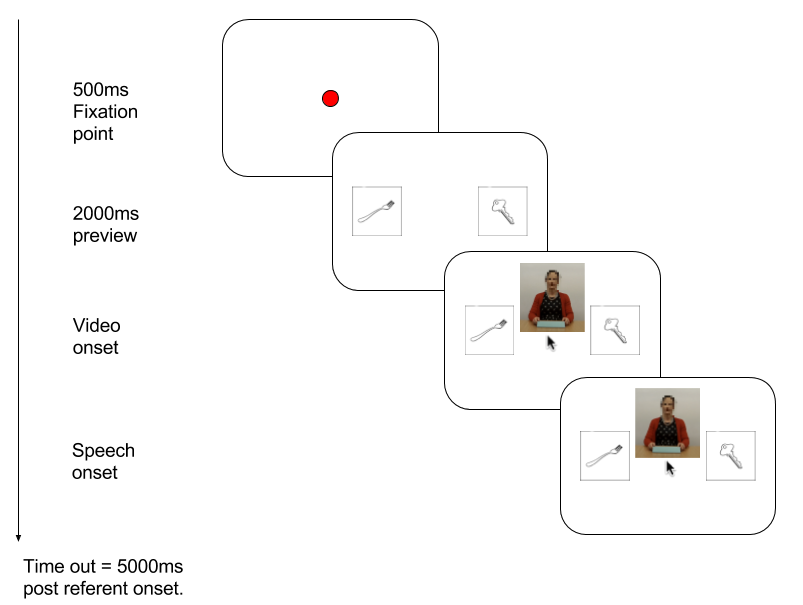
\includegraphics[width=\linewidth]{./img/e7_trial.png}
  \caption{Procedure of a given trial, Experiment 1}
  \label{fig:v1_trial}
\end{figure}
Between trials, participants underwent a manual drift correct, after which the fixation dot turned red for 500ms. 
After this, the two objects (referent and distractor) were displayed on the screen for 2000ms.
The video then appeared and the cursor was centred and made visible.
Playback of the utterance began after the variable speech onset associated with each video (Mean = 1410ms, SD = 410 ms). 
%After a given time (M=1410ms, sd=410ms), the utterance began. 

The instructions emphasised that the videos participants saw were recorded from a previous experiment, in which the speaker had to describe the location of some hidden treasure with the aim of misleading the listener into choosing the wrong location %in which one participant had to deceive another as to the location of some hidden treasure.
Participants were instructed to click on the object behind which \textit{they believed} the treasure to be hidden, with the overall aim of accumulating as much treasure as they could across the experiment.
Participants received no feedback after their object clicks, except on bonus filler trials, which are described in the next section.

% Jia: moved this here from the section below because it isn't directly releant to Bonus Rounds

Participants completed five practice trials (one of which was presented as a bonus round) prior to the main experiment. 
Two of these were static, two displayed the speaker in different postures, and one displayed the speaker making a trunk movement.

\subsection{Bonus Rounds}
To maintain motivation throughout the study, participants were told that there were a number of ``hidden bonus rounds'' which offered more treasure than regular rounds.
25\% of filler trials (half in the gesture condition; half in the no-gesture condition) were randomly designated as bonus rounds for each participant.
These trials were visually identical to regular trials, with the exception of a message informing participants that they had successfully located bonus treasure following their mouse click (regardless of the object chosen).

Participants were also told that the top scorers would be able to enter their names on a high-score table, which was shown at the beginning of the experiment. 

\subsection{Post-test Questionnaire}
Participants were asked to complete a short post-test questionnaire. 
The questionnaires contained three questions, the most important of which asked if participants noticed anything odd about the visual or audio stimuli.
Any participant who indicated that they noticed anything unusual was then verbally questioned, to decide whether they believed that the speech and gesture had been produced naturally and simultaneously.
All participants were subsequently debriefed (told that the audio and video were created separately and stitched together), and asked again verbally if they noticed anything unusual in that respect. 

\section{Results}
Twenty-four native English speaking participants took part in the experiment for a desired sample size of twenty. 
Participants were recruited from the University of Edinburgh community, and participated in return for a payment of \pounds{}4.
%Four participants who indicated suspicion of the proposed origins of the audiovisual stimuli, and their data was removed from all analysis.
Data from four participants who indicated suspicion of the proposed origins of the audiovisual stimuli based on the post-test questionnaire were removed from all analyses.

\subsection{Analysis}
Analysis was carried out in R version~3.4.4 \citep{Rbase2017}, using the lme4 package \citep{Bates2015}. 
Trials in which participants did not click on either the referent or distractor (0.003\% of trials) were excluded from all analyses. 

Object clicked (referent or distractor) was modeled using mixed effects logistic regression, with fixed effects of gesture type (No Gesture, Different Postures, Trunk Movements, Adaptor Gestures) and video-to-speech duration (Z-scored), thus controlling for any possible effect of perceived speech latency on judgments of dishonesty.
Random intercepts and slopes for gesture type and video-to-speech were included by-participant, along with random intercepts by-referent.
Reaction times (measured from referent onset) were modelled with the same fixed and random effect structure.
Following \citet{Lo2015}, we compared mixed effects logistic regression models which specified an identity link function, assuming gaussian, gamma and inverse gaussian distributions.

In previous studies using the treasure game paradigm, eye- and mouse- movements have been analysed over the time window starting at the onset of the referent name and extending for 800~ms; just beyond the duration of the longest referent (800~ms). % Jia: can't check right now but the duration of the longest referent (figure in brackets) was 700-and-something ms I think, not 800
Because the current study includes in the analysis all available referents (rather than the subset used in previous experiments), this window is extended to 0--1100~ms to include the duration of the longest referent (1062~ms) %the longest referent is 1062~ms, and so this window is extended to 1100~ms.

Eye fixation data was averaged into 20~ms bins (of 10 samples) prior to analysis.
For each bin, we calculated the proportions of time spent fixating referent or the distractor, resulting in a measure of the proportions of fixations on either object over time.

The position of the mouse was sampled every 40~ms.
Using the $X$ coordinates only, we calculated the number of screen pixels moved and the direction of movement (towards either referent or distractor).
We then calculated the cumulative distance travelled towards each object over time as a proportion of the cumulative distance travelled in both directions up until that time bin.
Movements beyond the outer edge of either object were considered to be `overshooting' and were not included in calculations (0.8\% of samples).
Eye- and mouse- biases were calculated from the proportions of referent to distractor fixations, and were subsequently empirical logit transformed \citep{Barr2008}. 
In these measures, a value of zero indicates no bias towards either object, and positive and negative values indicate a bias towards the referent and distractor respectively.

Eye and mouse data was modelled over the time window from 0 to 1100~ms post-referent onset using linear mixed effects models, with fixed effects of time, gesture type, and their interaction.
Random intercepts and slopes for time were included both by-referent and by-participant, along with by-participant random effects of gesture type.
Following \citet{Baayen2008}, we considered effects in these models to be significant where $|t|>2$.

% Jia: moved these sentences from above here so we're just talking about the regular elogit models first and then the growth curve models next, otherwise we seem to be going back and forth between describing the two
As visual inspection of the time-course of fixations towards either object suggested that there was a later effect of gestures in participants' decision of which object to click on, growth curve analysis (See \citealt{Mirman2008}) was used to investigate this further. 
This analysis was conducted over the time window from 0 to 1815~ms post-referent onset included 3 degrees of orthogonal polynomials for time, based on the pattern of the elogit referent-distractor bias having 2 turning points. 
These time polynomials, along with their interaction with gesture type, were included as fixed effects in a linear mixed effects model, with random intercepts and slopes for all time polynomials both by-participant and by-referent.


\subsection{Object clicks} % Jia: changed from 'mouse'->'object' for consistency with what we're calling it in the section above
Across the experiment, participants clicked on the referent in 55\% of trials and the distractor in only 45\%.
Table \ref{table:v1_clicks} shows the proportions of clicks to either object following different types of gesture.
When presented with an utterance accompanied by no-gesturing, participants showed a bias toward a final interpretation of the utterance as truthful, with more clicks to the referent than the distractor \resultsLog{0.62}{0.16}{<0.001}.
All types of gestures saw a reduction in this bias, with adaptor gestures (\resultsLog{-1.03}{0.34}{<0.005}) showing a greater change than different postures and trunk movements (\resultsLog{-0.72}{0.31}{<0.05} and \resultsLog{-0.62}{0.26}{<0.05} respectively). 
The duration of video shown prior to the beginning of speech was not found to be associated with which object was eventually clicked.

Comparisons --- via both AIC and BIC --- of reaction time models suggested that an inverse gaussian distribution provided the best fit to the observed data.
Neither gesture type nor duration of video prior to speech was associated with a significant change in reaction times.

\begin{table}
\caption{Object clicks}
\label{table:v1_clicks}
\begin{tabularx}{\linewidth}{YYYYY}
\hline
& No Gesture & Different Posture & Trunk Movement & Adaptor Gesture \\
Clicks to Referent & 63.8\% & 48.0\% & 49.7\% & 41.5\%  \\ 
Clicks to Distractor & 36.2\% & 52.0\% & 50.3\% & 58.5\% \\
\hline
\end{tabularx}
\end{table}

\subsection{Eye movements}
Figure \ref{fig:v1_eye} shows the time-course of fixations to referents and distractors over 2000~ms from referent onset, split by each type of video.

Analyses conducted over the period from referent onset to 1100~ms post-onset (duration of the longest referent) showed that, when presented with no gesture, participants displayed a fixation bias towards the referent which increased over time (\resultsLM{1.15}{0.29}{>2}).
For videos which presented the speaker either in a different posture, or producing an adaptor gesture, this increasing bias to the referent was significantly reduced
(\resultsLM{-0.97}{0.13}{>2}, \resultsLM{-0.59}{0.13}{>2}), but this was not the case for videos of trunk movements (\resultsLM{-0.25}{0.15}{=1.67}). 

Growth curve analysis over the period from referent onset to 1815~ms post-onset (mean click time) showed that when presented with no gesture, participants showed an tendency to fixate on the referent over the course of this time period (\resultsLM{0.67}{0.11}{>2}). %intercept term
Significant effects of gesture type on the intercept term indicated lower overall referent fixations during this period after viewing a different posture (\resultsLM{-0.36}{0.04}{>2}), a trunk movement (\resultsLM{-0.29}{0.4}{>2}), or an adaptor gesture (\resultsLM{-0.67}{0.4}{>2}), in comparison to the no gesture videos.
Significant interactions of gesture type and the linear time coefficient indicate that this reduction in referent-bias due to gesture type increases over the course of the window, with adaptor gestures showing a larger reduction relative to no gesture videos (\resultsLM{-116.89}{11.62}{>2}) than different postures (\resultsLM{-75.41}{11.65}{>2}) and trunk movements (\resultsLM{-58.78}{12.97}{>2}).
%Beyond this, different posture videos showed a more gradual initial tendency towards the referent relative to the no gesture videos (\resultsLM{39.83}{11.64}{>2}) and trunk movement videos showed an increased ??  (\resultsLM{33.50}{12.75}{>2}).
Figure \ref{fig:v1_gca} shows the time-course of the elogit referent-distractor bias, alongside the fitted values from the growth curve model. 

\begin{figure}[Ht]
  \centering
	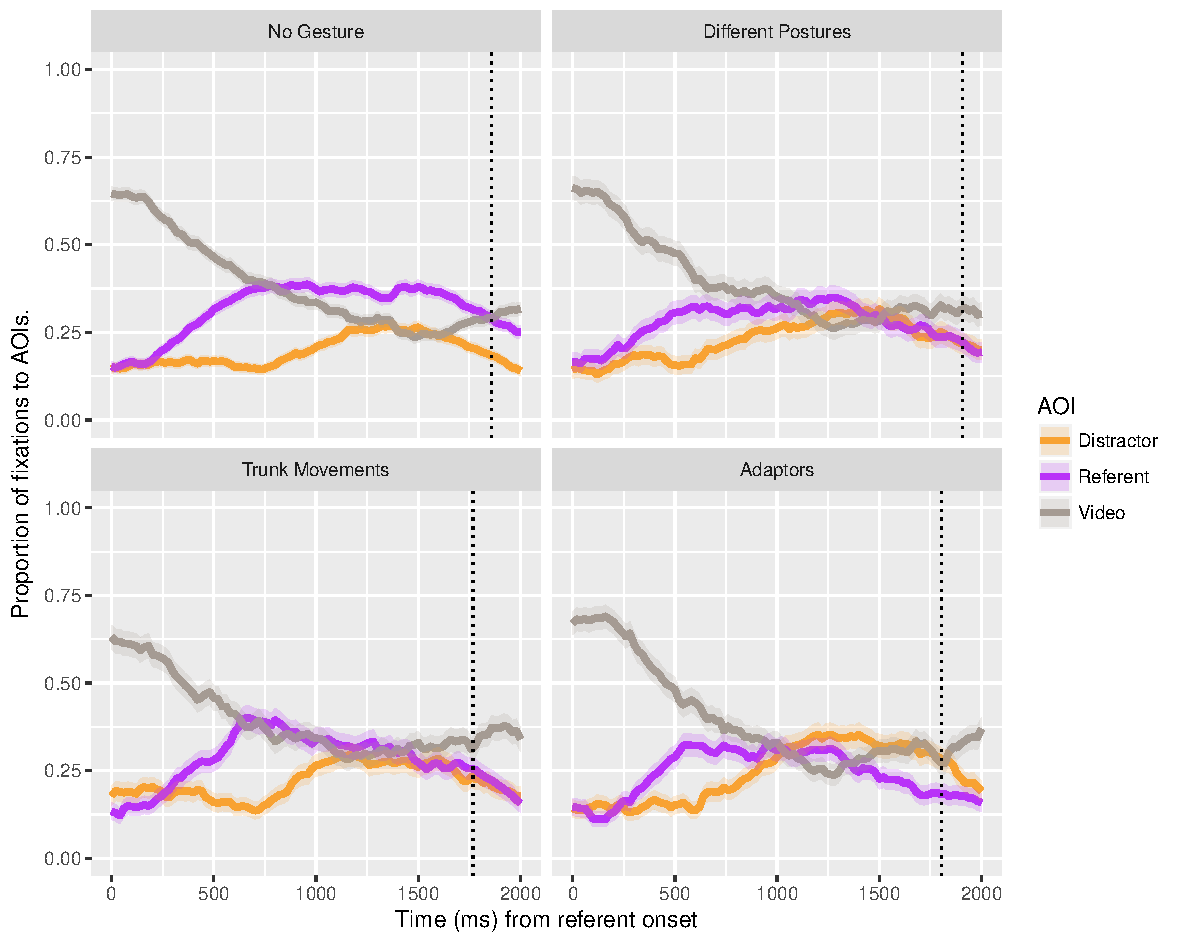
\includegraphics[width=\linewidth]{./img/e7_fixations.pdf}
  \caption{Eye-tracking results for Experiment 1: Proportion of fixations to each object (referent, distractor, video), from 0 to 2000 ms post-referent onset, calculated out of the total sum of fixations for each 20~ms time bin. Shaded areas represent $\pm$ 1 standard error of the mean.}
  \label{fig:v1_eye}
\end{figure}

\begin{figure}[Ht]
  \centering
	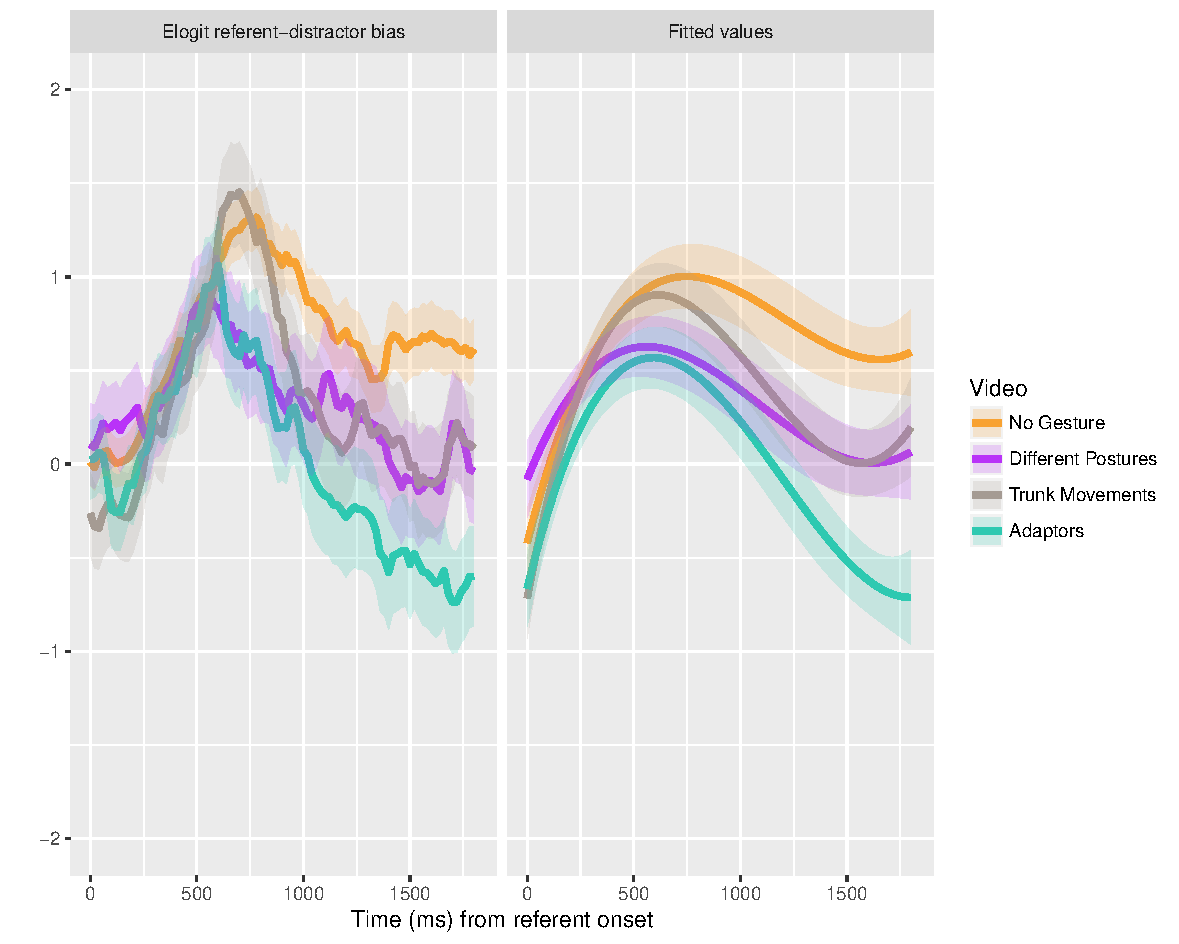
\includegraphics[width=\linewidth]{./img/e7_gcamodel.pdf}
  \caption{Elogit referent-distractor bias, and fitted values from growth curve analysis}
  \label{fig:v1_gca}
\end{figure}


\subsection{Mouse movements}
Figure \ref{fig:v1_mouse} shows the time-course of the proportions of cumulative distance the mouse moved towards the referent and distractor for 2000~ms from referent onset, split by each type of video.
Analysis on the time window from 0 to 1100~ms post-referent onset patterned with the eye-tracking data:
When the speaker made no gesture, participants showed a tendency to move increasingly towards referent over this period (\resultsLM{1.08}{0.22}{>2}).
As with eye-movements, different postures and adaptor gestures resulted in a weakening of this referent-bias (\resultsLM{-0.81}{0.13}{>2} and \resultsLM{-0.77}{0.13}{>2} respectively), but trunk movements did not (\resultsLM{-0.10}{0.14}{=0.69}). 

\begin{figure}[Ht]
  \centering
	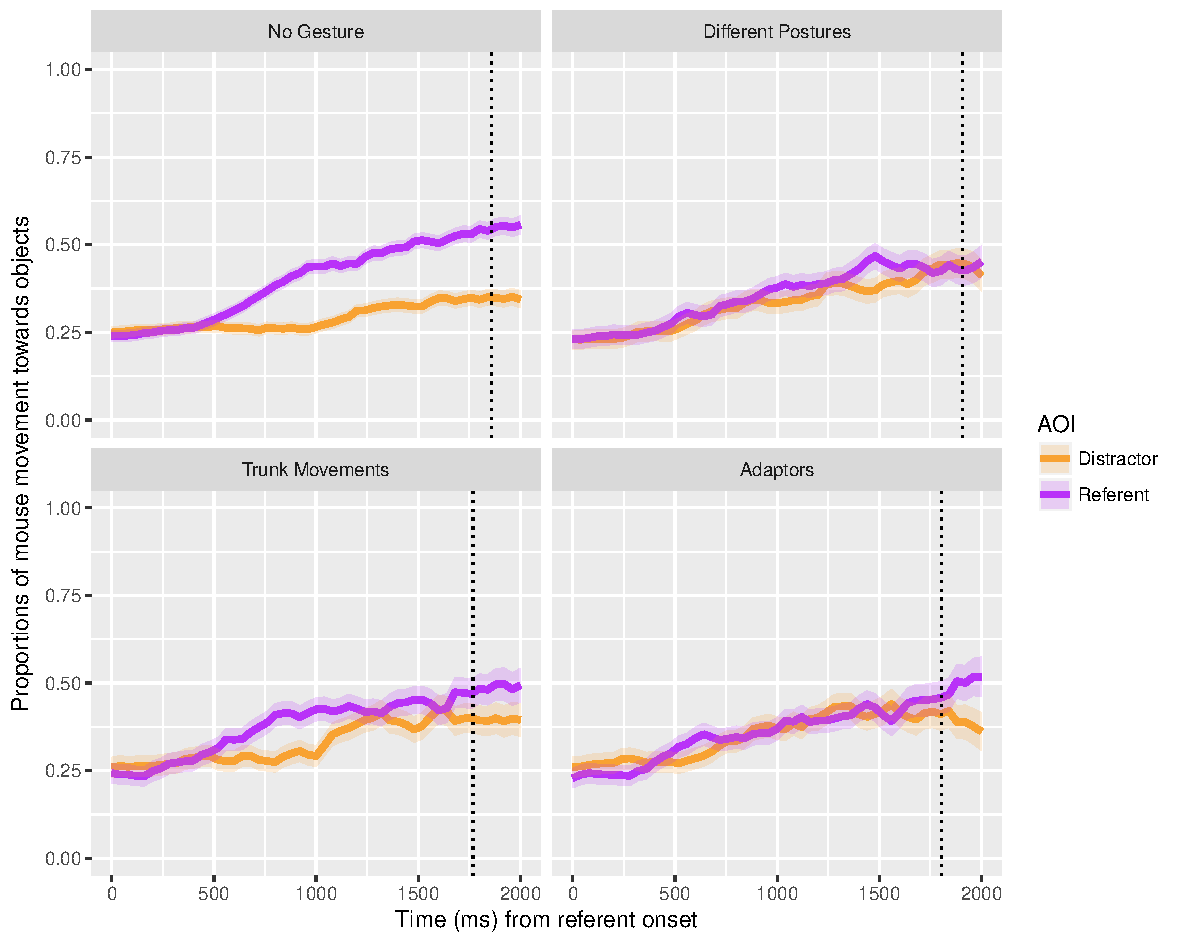
\includegraphics[width=\linewidth]{./img/e7_mouset.pdf}
  \caption{Mouse-tracking results for Experiment 2: Proportion of cumulative distance traveled toward each object from 0 to 2000 ms post-referent onset. Proportions were calculated from the total cumulative distance participants moved the mouse until that time bin (from video onset, when cursor was made visible). Shaded areas represent $\pm$ 1 standard error of the mean.}
  \label{fig:v1_mouse}
\end{figure}


\section{Discussion}
Experiment 1 investigated how the pragmatic inferences listeners make about a speaker's honesty are influenced by the presence of different types of movements and postures, and which of these provide the best means of studying the time-course of such inferences.
As in previous studies using this paradigm \citep{Loy2017, King2018}, participants showed a tendency to interpret an utterance as truthful when it had been presented without any potential cue to deceit.
Utterances presented alongside different postures and movements weakened this tendency, but only the presence of adaptor gesturing resulted in significantly more judgments of deception than truthfulness (indicated by clicks to the distractor over the referent).
The influence of the visual channel was also evident in the early stages of utterance processing, with videos of different postures and adaptor gestures resulting in a reduction of the tendency to fixate on --- and move the cursor toward --- the referent.
Interestingly, this early effect was not found for videos of trunk movements, perhaps a result of these gestures having been fully presented prior to the onset of speech, meaning that at the point of referent onset the audiovisual information immediately available to the listener was indiscernable from the no gesture videos. 
Similarities may be drawn here to the subtle differences when presented with either utterance-initial or utterance-medial speech disfluencies in \citet{Loy2017}: The temporal proximaty of a cue potentially influencing how much it reduces the initial referent-bias. 
% I know that you (jia) found no differences between experiments, but looking at the plots?
 
In contrast to previous versions of this paradigm, when presented with a possible cue to deception, the point at which listeners preference toward the referent tended to be matched (or overtaken, in the case of adaptor gestures) by the distractor was later, approximately 1000~ms post-referent onset. 
Contrastingly, participants in \citeauthor{Loy2017} showed little to no initial referent-bias following a disfluent utterance, with a distractor-bias appearing approximately 600~ms post-referent onset following both utterance-initial and utterance-medial disfluencies. 

There are several possible explanations for the later effect found in the current study.
Firstly, the inclusion of longer referents, along with the fact that not all referent-distractor pairs were controlled for phoneme onset, may result in establishing reference being delayed. 
Secondly, the visual component of the paradigm may be detracting from fixations to the two objects. 
This could also explain the differences in the early window (0 to 800~ms) between the types of gesturing: The reduction in the referent-bias may be a result of the video being more salient in both the different posture and the adaptor gesture conditions, and not evidence of the emerging gesture-lying bias.
That said, however, the initial referent-bias appears at approximately 300~ms post-referent onset in all conditions --- a point comparable to previous studies with this paradigm (\citealt{Loy2017, King2018}).

Lastly, it might be that the integration of gestural cues into judgments of deception is simply slower than it is for speech cues, taking longer to counteract the initial tendency to look at a named object. 
This is perhaps because the link from gestures to perceived deception might follow a different path than that from disfluency to deception.
\citet{Loy2017} showed that listeners' disfluency-lying bias occurs very early in comprehension, suggesting either a reliance upon a rule-of-thumb assocation between the two, or extremely fast inferential processing which links disfluency to deception via, for example, cognitive effort involved in planning a dishonest utterance (See \citealt{King2018}).
However, this might not be the case for gestures.
Speech disfluency can be mapped directly to the processes of speech production: It is a straightforward inferential link from the way a given utterance is delivered to the content of that utterance, be it pragmatic (e.g. lying) or literal (e.g. naming difficulty \citealt{Arnold2007}).
Co-speech movements, however, can map to many things, some only indirectly related to the production of speech, and some completely unrelated (e.g. scratching an itch).
Whilst there is evidence to suggest that cognitive effort increases gesturing \citep{Goldin-Meadow2001}, an alternative intuitive line of reasoning for a listener would, for instance, link gestures to nervousness/anxiety, and link nervousness to deception.
Indication of this can be found in the post-test questions which revealed that 4 participants felt that they had been responding to whether the speaker looked tense or relaxed (with 1 even mentioning that the movements looked more relaxed, and so signalled honesty).
In fact, only 2 participants explicitly linked an \textit{increase} in movement with lying; 9 mentioned using body language and gestures to make their judgments but specified neither rationale nor direction; and, oddly, 15 described perceiving differences in spoken delivery which they believed signalled lying (intonation, hesitancy). 
It might be that participants were not responding directly to the presence of a gesture, but to something which took longer to establish, such as how nervous the speaker looked over the course of the video.

The results from Experiment 1 support previous findings in the deception literature, indicating that listeners judgments of deception are influenced by different postures and gestures. 
However, it is possible that the time-course of these judgments was made less clear by stimuli which did not capture the underlying mechanism by which listeners associate gesture with lying.
To clarify this, we conducted Experiment 2, a simplified version of the experiment in which we focused on one type of gesturing, and in which, after completing the eye-tracking study, participants rated the videos on perceived anxiety.

\section{Experiment 2}
Experiment 2 focused on the influence of adaptor gestures on judgments of dishonesty, and looked at whether these judgments paralleled with perceptions of nervousness in the speaker.
If gesture is linked to deception via perceived anxiety, then gestures which are rated as more nervous should result in more judgements of dishonesty. 
Using the same paradigm as Experiment 1, participants in Experiment 2 saw utterances accompanied by either an adaptor gesture or no gesture.
After the eye-tracking task, participants then rated each video on how nervous the speaker looked.

\subsection{Materials}
A subset of 40 images from those in Experiment 1 were used across twenty trials.
As in Experiment 1, these images were presented in referent-distractor pairs, combined with 20 utterances naming the referent as the location of the treasure.
The referents and distractors used were those which, in \citet{Loy2017}, had been matched for both ease of naming and familiarity.

In Experiment 2, participants saw these pairs of images alongisde a selection of 10 Adaptor Gestures and 10 Static/No Gesture videos.
Based on participant feedback from Experiment 1, care was taken to ensure that the No Gesture videos presented the speaker in a relaxed posture. 
Adaptor gestures were based on descriptions of anxious non-verbal behaviour from \citet{Gregersen2005}.
Prior to running the study, 28 videos (18 different adaptor gestures, 10 static) were rated on how nervous the speaker looked.
10 native english speakers were told that they were going to watch videos (without audio) of someone being questioned in a stressful situation, and were asked to rate how nervous the speaker looked in each video (1: very relaxed, 7: very nervous). 
The 10 adaptor gestures with the highest ratings (Mean = 4.1, SD = 1.5) were included in the experiment, along with the 10 static recordings (M = 1.9, SD = 1.1).

The 20 referents were counterbalanced across two lists such that each referent that occurred with a gesture in the first list occurred without a gesture in the second.
The pairings of referents with specific videos/gestures within each condition was randomised on each run of the experiment.

One key difference from Experiment 1 was that speech initiation time (the duration from video onset to speech onset) in Experiment 2 was a fixed constant: In all trials, speech began 1170~ms after the beginning of the video.
There were no other procedural differences in trials between experiments 1 and 2, and no trials in Experiment 2 displayed a bonus round message. 

After the main task, participants were asked to watch the videos again, without audio, rating how nervous they thought the speaker looked (using the same 1-7 scale as described above).
Participants then completed the same post-test questionnaire as in Experiment 1, with data being excluded from analysis based on the same criteria.

\section{Results}
Twenty-three native English speaking participants took part, with three participants excluded due to suspicion of the audiovisual stimuli being scripted.
Participants were paid \pounds{}3.

\subsection{Analysis}
We followed the same analysis strategy as was used for Experiment 1, with the experimental manipulation of gesture being a dichotomous Gesture vs.\@ No Gesture.
Trials which did not result in a click to either object (0.8\%) were excluded, along with mouse movements beyond the outer edge of the objects (1\% of samples).

Analyses of object clicks and reaction times did not control for video-to-speech duration, since this was controlled in the experimental design.
To investigate whether listeners deception judgments were predicted by their subsequent ratings of perceived nervousness, analysis of object clicks included participants' post-test ratings (Z scored) of each video as a fixed effect, along with the interaction with gesture.

The time window of analysis for eye- and mouse- movements was reduced to the 800~ms following referent onset, based on the fact that the subset of referents included in this experiment had a maximum duration of 776~ms. 
Because Experiment 2 fully counterbalanced gesture across all referents, random effects of gesture and time and their interaction were included both by-referent and by-participant.

\subsection{Mouse clicks}
Across the experiment, participants clicked on the referent in 53\% of trials and the distractor in 47\%.
Table \ref{table:v2_clicks} shows the proportions of clicks to either object following videos displaying either an adaptor gesture or no gesture.
As in experiment 1, participants showed a bias toward a final interpretation of the utterances without gestures as truthful, with more clicks to the referent than the distractor \resultsLog{1.15}{0.37}{<0.005}.
Patterning with the adaptor gestures in experiment 1, utterances presented with an adaptor gesture resulted in bias towards clicking the distractor (\resultsLog{-2.45}{0.51}{<0.001}).
Inclusion of participants post-test ratings of how nervous they perceived the speaker to be in each video did not improve model fit (${\chi}^2$=0.46)
There was no effect of gesture on time to click.

\begin{table}
\caption{Object clicks}
\label{table:v2_clicks}
\begin{tabularx}{\linewidth}{YYY}
\hline
& No Gesture & Gesture \\
Clicks to Referent & 80.9\% & 24.2\%  \\
Clicks to Distractor & 19.1\% & 75.8\%  \\
\hline
\end{tabularx}
\end{table}


\subsection{Eye movements}
Figure \ref{fig:v2_eye} shows the time-course of fixations to referents and distractors over 2000~ms from referent onset, split by presence of gesture.
Analyses conducted over the period from referent onset to 800~ms post-onset patterned with results from Experiment 1: 
When presented with an utterance unnaccompanied by gesture, participants displayed a fixation bias towards the referent which increased over time (\resultsLM{3.03}{0.77}{>2}).
When presented with an utterance accompanied by an adaptor gesture, this bias was greatly reduced (\resultsLM{-3.00}{1.02}{>2}).

\begin{figure}[Ht]
  \centering
	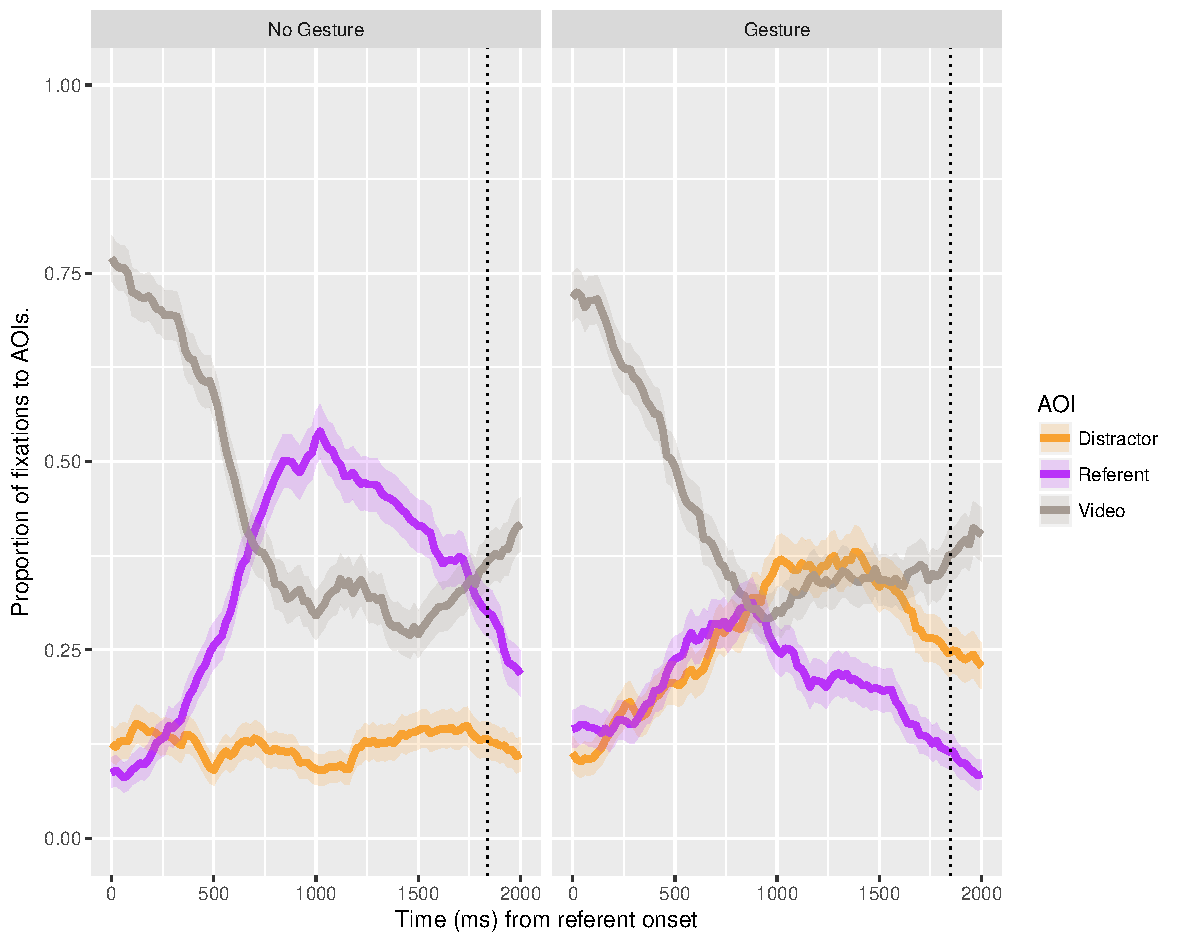
\includegraphics[width=\linewidth]{./img/e8_fixations.pdf}
  \caption{Eye-tracking results for Experiment 2: Proportion of fixations to each object (referent, distractor, video), from 0 to 2000 ms post-referent onset, calculated out of the total sum of fixations for each 20~ms time bin. Shaded areas represent $\pm$ 1 standard error of the mean.}
  \label{fig:v2_eye}
\end{figure}



\subsection{Mouse movements}
Figure \ref{fig:v2_mouse} shows the time-course of the proportions of cumulative distance the mouse moved towards the referent and distractor for 2000~ms from referent onset, split by presence of gesture.
Analysis on the period from 0 to 800~ms post-referent onset patterned with the eye-tracking data:
Following no gesture videos, participants showed a tendency to move increasingly towards referent over this period (\resultsLM{1.90}{0.39}{>2}).
As with eye-movements, this referent-bias was greatly reduced following a gesture (\resultsLM{-2.46}{0.77}{>2})

\begin{figure}[Ht]
  \centering
	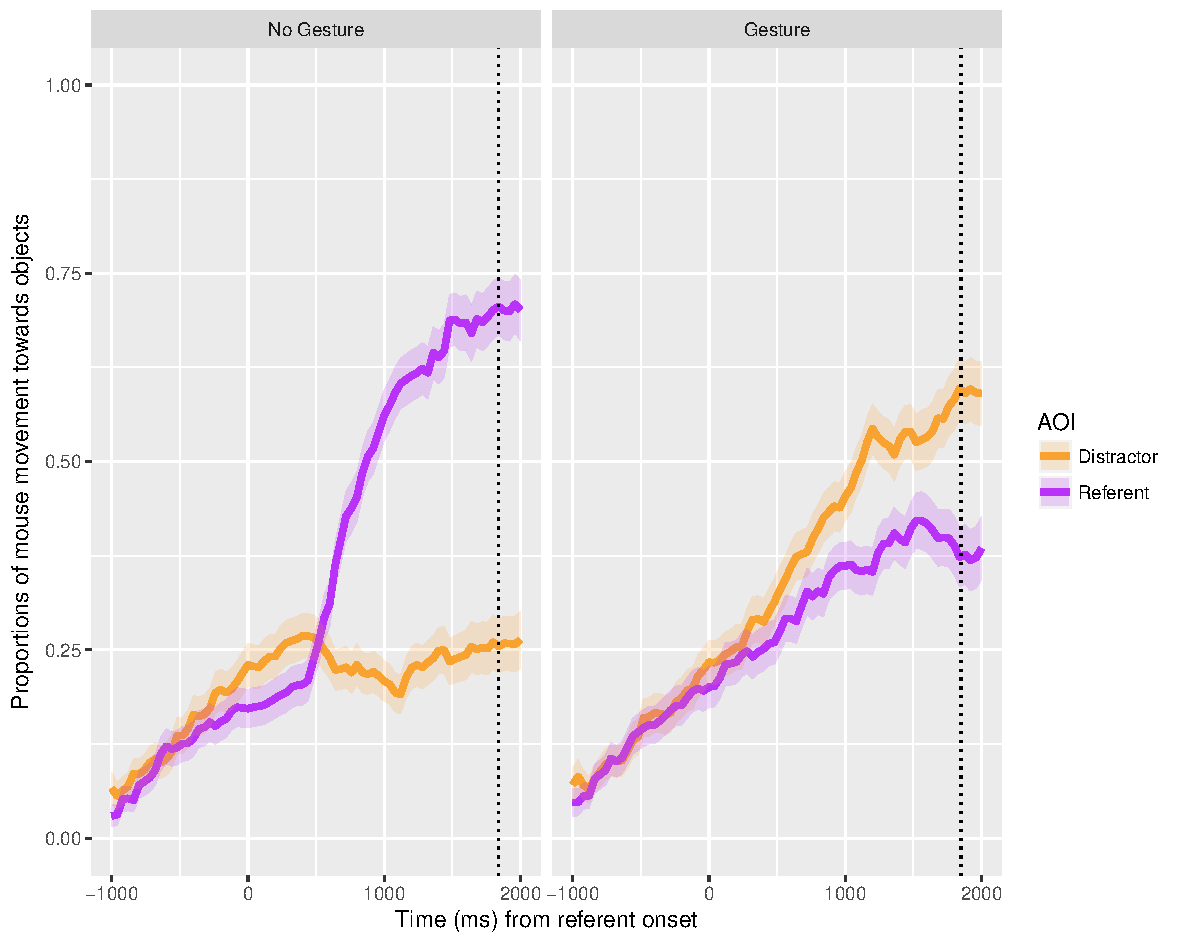
\includegraphics[width=\linewidth]{./img/e8_mouset.pdf}
  \caption{Mouse-tracking results for Experiment 2: Proportion of cumulative distance traveled toward each object from 0 to 2000 ms post-referent onset. Proportions were calculated from the total cumulative distance participants moved the mouse until that time bin (from speech-onset, when cursor was made visible). Shaded areas represent $\pm$ 1 standard error of the mean.}
  \label{fig:v2_mouse}
\end{figure}

\section{Discussion}
Across both experiments, participants showed a slight overall tendency to take an utterance as honest rather than dishonest, although this only differed from chance in Experiment 1. 
Our results show that the body language and gestures which accompany a spoken utterance affects the judgments which listeners make about the utterance's veracity.
Utterances presented with a comparatively neutral posture and no gesturing bias listeners towards believing the speaker to be truthful, as shown by increased tendency to fixate on, and move towards, the object which was named by the speaker. 
Comparable to fluent (as opposed to disfluent) utterances in \citet{Loy2017}, this implicit honesty-bias when faced with no obvious potential cue is consistent with previous research in detecting actual lies from truths, which suggest a general tendency to judge a speaker as truthful (\citealt{Vrij2000}).

Consistent with previous research in deception judgments and beliefs about deceptive cues, participants linked dishonesty with an increase in movement. 
As in \citet{Loy2017}, the pragmatic judgments which listeners made began during the on-line processing of speech, becoming apparent alongside the unfolding of the critical linguistic input.
The speed with which these judgments were made --- especially in Experiment 2 --- suggest that visual information can modulate listeners' judgments about a speaker's intentions concurrently with the integration of lexical information.

Different types of gestures and postures influence deception judgments to different degrees, affecting the time-course of these judgments accordingly. 
A reduction in the tendency to believe the speaker was apparent when the speaker was either in a different posture or made a trunk movement prior to speaking, although these resulted in no final tendency towards interpretations of either honesty or dishonesty. 
Only utterances presented with adaptor gesturing were associated with more judgements of dishonesty than of truthfulness, and this patterned with the greatest reduction in the early eye- and mouse- movement biases towards the referent. 
Experiment 2 provided a clearer account of the influence of adaptor gestures on deception judgments at the early moments of referent comprehension, with the tendency to look --- and move --- towards the referent being completely attenuated when the utterance was presented with a gesture. 
However, following adaptor gestures in both experiments, the bias towards the distractor --- signifying perceived dishonesty --- over the referent appeared approximately 1000~ms after the referent began, at a later point than previous versions of this paradigm have found speech disfluency to modulate deception judgments.
This may be simply due to listeners associating lying with \textit{any} disfluency, only \textit{some} gestures.
To better understand how cues to deception in different modalities differ, further research would require investigating the effect of disfluency when the visual channel is also available --- for example, studying the time course of deception judgments when faced with one or both of a disfluency and an adaptor gesture. %i.e. GVD

Interestingly, participant's subsequent ratings of how nervous the speaker looked in each video did not pattern with their final judgments beyond whether or not the video presented a gesture, suggesting that listeners' associations between gesture and lying is not necessarily a consequence of perceived anxiety in the speaker.
Although the mechanism behind listeners' associations between gestures and deception remain unclear, our results show that gestural cues influence pragmatic judgments at the early stages of comprehension, but suggest that the integration of these cues to inform deception judgments might be more gradual than the integration of spoken cues.



\bibliography{./GCD}

\end{document}
